\chapter{Numerical Analysis}
\label{ch:Num}
In this chapter we will discuss numerical methods for solving stochastic differential equations based on the stochastic Taylor expansions which have been presented in section \ref{stochasticTaylor}. These are also called \emph{time discrete approximations} since we will give the approximative values on points of the time interval [0,T]. We will consider strongly converging schemes only. Strong means in this context that we want to approximate the \emph{sample paths} of the true solution \(X_t\) of a stochastic differential equation. On the other hand, weakly converging schemes deal with the approximation of some funcionals of the true solution \(X_t\), for example the expected value or the variance. Obviously, strongly converging schemes are also weakly converging.\\
These methods will be discussed: \emph{Euler-Maruyama-scheme} and the \emph{Milstein-scheme}.\footnote{There is a third method which we also implemented: the \emph{Wagner-Platen-scheme}, but we will not give a discussion of this scheme and refer to \cite{KloedenPlaten} for the details, the scheme is also called \emph{order 1.5 strong stochastic Taylor scheme} and it is also based on the stochastic Taylor expansion. See appendix \ref{code} for the implementations and appendix \ref{Graphics} for graphics.}
We will prove the convergence of these methods and give the convergence order analytically. In the final sections of this chapter we will discuss the results and determine the convergence order numerically using simulations.


\section{Strong convergence and error analysis}
\label{erroranalysis}
For the moment, let us consider a general setting. Let \(X_t\) be the solution of a stochastic differential equation and let  \(\overline{X}_{t}\) denote its approximation on [0,T].  
We want that the sample paths on [0,T] of the approximation are close to the sample paths of the true solution (pathwise approximation).
There are many different criterions to measure the closeness or the approximation error:
\begin{enumerate}[noitemsep,topsep=0mm,labelindent=6mm,leftmargin=*,widest=3.,align=right]
\item \(\mathbb{E}[|X_T - \overline{X}_{T}|]\quad\) (absolute error at T)
\item \(\mathbb{E}[(X_T - \overline{X}_{T})^2]^{\frac{1}{2}}\quad\) (squared-mean error at T)
\item \(\sup_{t\in[0,T]}\mathbb{E}[|X_t - \overline{X}_{t}|]\quad\) (uniform absolute error)
\item \(\sup_{t\in[0,T]}\mathbb{E}[(X_t - \overline{X}_{t})^2]^{\frac{1}{2}}\quad\) (uniform squared-mean error)
\end{enumerate}
The first two criterions measure the error at the final time-point T. We will use the second criterion in our numerical simulations, since it is a bound for the absolute error at T: \(\mathbb{E}[|X_T - \overline{X}_{T}|]\leq\mathbb{E}[(X_T - \overline{X}_{T})^2]^{\frac{1}{2}}\) and the implementation is simple. We assume that the approximation error is determined at the final time point T. However we will use the uniform squared-mean error criterion in our convergence proofs.

Now let \(\overline{X}^{n}_{t}\) define a sequence of approximate solutions on partitions \(P_n\) of [0,T]. This means for each n we have a time-grid with n steps and step-size \(\frac{T}{n}\).
Now define the approximation error \(e_n\) for each n:
\[e_n\coloneqq\mathbb{E}[(X_T - \overline{X}^{n}_{T})^2]^{\frac{1}{2}}.\]
Obviously we want that \(e_n\to 0\) as \(n\to\infty\) holds for our approximation schemes. However for practical applications we are interested in how fast different approximation schemes converge to the true solution \(X_t\) for increasing n (where we use the criterion as norm).
We want also to be able to compare different approximation schemes regarding their convergence speed. 

Let us consider the following definition:
\begin{definition}[Strong convergence and strong convergence order]
The approximation \(\overline{X}^n_{t}\) converges to \(X_t\) in the strong sense if there are constants K and \(\gamma > 0\) s.t:
\[e_n \leq K\cdot n^{-\gamma}\]
The convergence speed is determined by \(\gamma\). Thus we will call \(\gamma\) the \emph{strong order of convergence} and we will say that \(\overline{X}^n_{t}\) converges strongly with order \(\gamma\) to the true solution \(X_t\) for increasing n.
\end{definition}

It will be important to have an estimate for \(\gamma\) for our approximation schemes. This can be given either analytically or empirically through simulation. We will discuss both.
For the empirical estimation we can justify heuristically:
\begin{flalign*}
&\log(e_n) = \log(K) -\gamma\log(n) &\\
&\log(e_{n+1}) = \log(K) -\gamma\log(n+1) &\\
&\log(e_{n+1}) - \log(e_n) = -\gamma\cdot(\log(n+1)-\log(n)) &\\
&\frac{\log(e_{n+1}) - \log(e_n)}{\log(n+1) - \log(n)}= -\gamma &
\end{flalign*}
We can plot the points (\(\log(n),\log{(e_n)}\)) for all our n and draw a regression line. The slope of the line is then an estimate for \(-\gamma\).
In our simulations we will choose the values of n to be powers of 2. This will allow us to use the refinement algorithm for the discretizations, see algorithm \ref{alg:Refinement}. In this case it makes sense to take the logarithm to base 2.


\section{Strongly converging schemes}
In this section we will present the Euler-Maruyama-scheme and the Milstein-scheme. Both schemes can be constructed by truncating stochastic Taylor expansions, which have been discussed in section \ref{stochasticTaylor}. 
We will give the algorithm and prove their convergence properties. We will show that the Euler-scheme has strong order of convergence 0.5, and the Milstein-scheme has strong order of convergence 1 under some conditions on the coefficients.

Let us fix the following setting.
We have given a stochastic differential equation:
\begin{flalign*}
& \mathrm{d}X_t = a(X_t)\mathrm{d}t + b(X_t)\mathrm{d}W_t,\quad t\in[0,T],\quad X_0 = x_0\\
& X_t = x_0 + \int_0^t \!a(X_s)\,\mathrm{d}s + \int_0^t \!b(X_s)\,\mathrm{d}W_{s} \quad\text{P-a.s.}
\end{flalign*}
where the functions \(a:\mathbb{R}\mapsto\mathbb{R}\), \(b:\mathbb{R}\mapsto\mathbb{R}\) and the initial value \(x_0\) are defined as in \ref{Itoprocess}, and fulfill the properties of \ref{lemma:ExUn}. 
Especially \(x_0\) is square-integrable. Then since \(X_t\in L_2[\Omega]\), \(\mathbb{E}[X_t^2]<\infty\:\:\forall t\in[0,T]\).\\
Let \(X_t:[0,T]\times\Omega\mapsto\mathbb{R}\) be the unique solution process of the stochastic differential equation.
Let [0,T] be a time interval, T finite. Let \(P_n = \{t_0=0,\dots, t_n\coloneqq T\}\) be a discretization of [0,T] with n steps and constant stepsize \(\frac{T}{n}\).
Let \(\overline{X}^n_{t_k}\) denote the approximative solution (for given step-amount n) on the grid-points \(t_k\) for k = 0,\dots,n.

\subsection{Euler-Maruyama-scheme}
The Euler-Maruyama-scheme can be obtained from the 1. stochastic Taylor expansion, see proposition \ref{prop:stochTaylor1}, by giving the expansion for each \([t_{k}, t_{k+1}],\:k=0,\ldots,n-1\), and by truncating the remainder term.
\begin{algorithm}[Euler-Maruyama-scheme]
\begin{enumerate}[noitemsep,topsep=0mm,labelindent=6mm,leftmargin=*,widest=3.,align=right]
\item Initialize \(\overline{X}^n_{t_0}=x_0\)
\item For k = 0 to n-1
\begin{enumerate}[noitemsep,topsep=0mm,labelindent=6mm,leftmargin=*,widest=3.,align=right]
\item Generate \(\triangle\!W_k \sim \mathcal{N}(0,\frac{T}{n})\)
\item Set \(\overline{X}^n_{t_{k+1}} = \overline{X}^n_{t_k} + a(\overline{X}^n_{t_k})\triangle\!t_k + b(\overline{X}^n_{t_k})\triangle\!W_k\)
\end{enumerate}
\item Linear interpolation.
\end{enumerate}
Where \(\triangle\!t_k\coloneqq t_{k+1}-t_k=\frac{T}{n}\) and \(\triangle W_k = W_{t_{k+1}}-W_{t_{k}}\sim\mathcal{N}(0,\frac{T}{n})\) for k=0,\dots,n-1.

This algorithm gives us values of the approximation on the discretization points and we can use linear interpolation if needed.
\end{algorithm}

\begin{theorem}[Strong convergence of the Euler-Maruyama-scheme]
Let \(L_a\), \(L_b\) be constants. 
Let \(a:\mathbb{R}\mapsto\mathbb{R}\) and \(b:\mathbb{R}\mapsto\mathbb{R}\) satisfy \(\forall x,y\in\mathbb{R}\):
\begin{enumerate}[noitemsep,topsep=0mm,labelindent=6mm,leftmargin=*,widest=3.,align=right]
\item \(|a(x) - a(y)| \leq L_a|x-y| \\
	    |b(x) - b(y)| \leq L_b|x-y|\)	
\item \(a(x)^2 \leq C(1+x^2) \\
	    b(x)^2 \leq C(1+x^2) \)
\end{enumerate}
Let \(\overline{X}^n_{t_{k}}\) be an Euler-Maruyama approximation of the above equation for k = 0,\(\dots\),n with step size \(\frac{T}{n}\).
Let \(\overline{X}^n_{t}\) be the constant extension\footnote{It is also possible to take linear interpolation instead, however the proof is simpler this way.} of the approximation. This means we will define:
\[\overline{X}^n_{t}\coloneqq\overline{X}^n_{t_{k}}\quad\text{for}\:\:t\in[t_k,t_{k+1})\]
then:
\[\sup_{t\in[0,T]}\mathbb{E}[(X_t-\overline{X}^n_{t})^2]^{\frac{1}{2}} = \sup_{t\in[0,T]}\|X_t-\overline{X}^n_{t}\|_{L^2[\Omega]}\leq K\cdot n^{-\frac{1}{2}}\]
for some constant K.
\end{theorem}
This means that the Euler-Maruyama approximation is converging strongly in \(L_2[\Omega]\) to the true solution process with order 0.5 for t\(\in\![0,T]\). This is an uniform error-bound since the bound does not depend on t.
\begin{proof}
Fix t\(\in[t_k,t_{k+1}]\). Then:
\begin{flalign*}
\|X_t-\overline{X}^n_{t}\|_{L^2[\Omega]} & = \|\int_0^t \!a(X_s)\,\mathrm{d}s + \int_0^t \!b(X_s)\,\mathrm{d}W_{s} -\int_0^{t_k} \!a(\overline{X}^n_{s})\,\mathrm{d}s - \int_0^{t_k} \!b(\overline{X}^n_{s})\,\mathrm{d}W_{s}\|_{L^2[\Omega]}&\\
										&= \|\int_{t_{k}}^t \!a(X_s)\,\mathrm{d}s + \int_0^{t_k} \!a(X_s)-a(\overline{X}^n_{s})\,\mathrm{d}s&\\
										& + \int_{t_{k}}^t \!b(X_s)\,\mathrm{d}W_{s} + \int_0^{t_k} \!b(X_s)-b(\overline{X}^n_{s})\,\mathrm{d}W_{s}\|_{L^2[\Omega]}.&\\
										& \leq \|\int_{t_{k}}^t \!a(X_s)\,\mathrm{d}s\|_{L^2[\Omega]} + \|\int_0^{t_k} \!a(X_s)-a(\overline{X}^n_{s})\,\mathrm{d}s\|_{L^2[\Omega]}&\\
									 	& + \|\int_{t_{k}}^t \!b(X_s)\,\mathrm{d}W_{s}\|_{L^2[\Omega]} + \|\int_0^{t_k} \!b(X_s)-b(\overline{X}^n_{s})\,\mathrm{d}W_{s}\|_{L^2[\Omega]}.&
\end{flalign*}
Where we used the triangle-inequality.\\
Now we will take the square and use: \\
\((a+b+c+d)^2\leq 4(a^2+b^2+c^2+d^2)\quad\forall a,b,c,d\in\mathbb{R}\).
\begin{flalign*}
\|X_t-\overline{X}^n_{t}\|_{L^2[\Omega]}^2 & \leq	 4(\|\int_{t_{k}}^t \!a(X_s)\,\mathrm{d}s\|_{L^2[\Omega]}^2 + \|\int_0^{t_k} \!a(X_s)-a(\overline{X}^n_{s})\,\mathrm{d}s\|_{L^2[\Omega]}^2\\
									 	    & + \|\int_{t_{k}}^t \!b(X_s)\,\mathrm{d}W_{s}\|_{L^2[\Omega]}^2 + \|\int_0^{t_k} \!b(X_s)-b(\overline{X}^n_{s})\,\mathrm{d}W_{s}\|_{L^2[\Omega]}^2)\\
\end{flalign*}
Now let us estimate each integral separately.
\begin{align*}
\|\int_{t_{k}}^t \!a(X_s)\,\mathrm{d}s\|_{L^2[\Omega]}^2 & = \mathbb{E}[(\int_{t_{k}}^t \!a(X_s)\,\mathrm{d}s)^2] \, \leq \mathbb{E}[\int_{t_{k}}^t \!a(X_s)^2\,\mathrm{d}s\cdot\int_{t_{k}}^t \!\,\mathrm{d}s] &\\
													      & \leq \frac{T}{n}\int_{t_{k}}^t\!\mathbb{E}[a(X_s)^2]\,\mathrm{d}s  \leq C\cdot\frac{T}{n}\int_{t_{k}}^t\!\mathbb{E}[1+X_s^2]\,\mathrm{d}s &\\
													      & \leq C\!\cdot\!(\frac{T}{n})^2\!\cdot\!M &	
\end{align*}
where \(M\coloneqq\sup_{s\in[0,T]}\mathbb{E}[1+X_s^2]<\infty\).\\
We used Cauchy-Schwarz, Fubini and the linear growth-bound.																																														
\begin{flalign*}
\|\int_0^{t_k} \!a(X_s)-a(\overline{X}^n_{s})\,\mathrm{d}s\|_{L^2[\Omega]}^2 & = \mathbb{E}[(\int_0^{t_k}\!a(X_s)-a(\overline{X}^n_{s})\,\mathrm{d}s)^2]& \\
																		    & \leq \mathbb{E}[\int_0^{t_k}\!(a(X_s)-a(\overline{X}^n_{s}))^2\,\mathrm{d}s\cdot\int_0^{t_k}\!\,\mathrm{d}s] &\\
																		    & \leq T\cdot L_a^2\cdot \int_0^{t_k}\!\mathbb{E}[(X_s-\overline{X}^n_{s})^2]\,\mathrm{d}s&
\end{flalign*}
We used again Cauchy-Schwarz, Fubini and the Lipschitz-condition.
\begin{flalign*}
\|\int_{t_{k}}^t \!b(X_s)\,\mathrm{d}W_{s}\|_{L^2[\Omega]}^2 & = \mathbb{E}[(\int_{t_{k}}^t \!b(X_s)\,\mathrm{d}W_{s})^2]  = \mathbb{E}[\int_{t_{k}}^t \!b(X_s)^2\,\mathrm{d}s] &\\
															& = \int_{t_{k}}^t \! \mathbb{E}[b(X_s)^2]\,\mathrm{d}s\,\,\,\,\,\,\,\,\,\,      \leq C \int_{t_{k}}^t \! \mathbb{E}[1+X_s^2]\,\mathrm{d}s&\\
															& \leq C\!\cdot\!\frac{T}{n}\!\cdot\!M&
\end{flalign*}
We used the It\^o-isometry, Fubini and the linear growth-bound.	
\begin{flalign*}
\|\int_0^{t_k} \!b(X_s)-b(\overline{X}^n_{s})\,\mathrm{d}W_{s}\|_{L^2[\Omega]}^2 & = \mathbb{E}[(\int_0^{t_k}\!b(X_s)-b(\overline{X}^n_{s})\,\mathrm{d}W_{s})^2] &\\
																				& =  \mathbb{E}[\int_0^{t_k}\!(b(X_s)-b(\overline{X}^n_{s}))^2\,\mathrm{d}s] &\\
																				& =  \int_0^{t_k}\!\mathbb{E}[(b(X_s)-b(\overline{X}^n_{s}))^2]\,\mathrm{d}s &\\ 
																				& \leq L_b^2\cdot\int_0^{t_k}\!\mathbb{E}[(X_s-\overline{X}^n_{s})^2]\,\mathrm{d}s&
\end{flalign*}
We used again the It\^o-isometry, Fubini and the Lipschitz-condition.\\
We just showed:
\begin{flalign*}
\|X_t-\overline{X}^n_{t}\|_{L^2[\Omega]}^2 & \leq	 4CM\frac{T}{n}(1+\frac{T}{n}) + 4(TL_a^2+L_b^2)\int_0^{t_k}\!\|X_s-\overline{X}^n_{s}\|_{L^2[\Omega]}^2\,\mathrm{d}s&\\
										    & \leq 4CM\frac{T}{n}(1+\frac{T}{n}) + 4(TL_a^2+L_b^2)\int_0^{t}\!\|X_s-\overline{X}^n_{s}\|_{L^2[\Omega]}^2\,\mathrm{d}s&
\end{flalign*}
Since t\(\in[t_k,t_{k+1}]\).\\
Now we will use the Gronwall-inequality, see appendix \ref{Gronwall}. This gives us:
\begin{flalign*}
\|X_t-\overline{X}^n_{t}\|_{L^2[\Omega]}^2 \leq 4CM\frac{T}{n}(1+\frac{T}{n})\!\cdot\!\exp(4T(TL_a^2+L_b^2))&
\end{flalign*}
Now we will use that a term of the form: \(\frac{C_1}{n} + \frac{C_2}{n^2}\) can be estimated by \(\frac{C_3}{n}\) from above for some constants.
Taking the square-root gives us: 
\begin{flalign*}
\|X_t-\overline{X}^n_{t}\|_{L^2[\Omega]} \leq K\cdot n^{-\frac{1}{2}}
\end{flalign*}
for some constant K and  t\(\in\![0,T]\).
This completes the proof.
\end{proof}

\subsection{Milstein-scheme}
The Milstein-scheme can be obtained by truncating the remainder term of the 2. stochastic Taylor expansion, see proposition \ref{prop:stochTaylor2}.
\begin{algorithm}[Milstein-scheme]
\begin{enumerate}[noitemsep,topsep=0mm,labelindent=6mm,leftmargin=*,widest=3.,align=right]
\item Initialize \(\overline{X}^n_{t_0}=x_0\)
\item For k = 0 to n-1
\begin{enumerate}[noitemsep,topsep=0mm,labelindent=6mm,leftmargin=*,widest=3.,align=right]
\item Generate \(\triangle\!W_k \sim \mathcal{N}(0,\frac{T}{n})\)
\item Set \(\overline{X}^n_{t_{k+1}} = \overline{X}^n_{t_k} + a(\overline{X}^n_{t_k})\triangle\!t_k + b(\overline{X}^n_{t_k})\triangle\!W_k\\
+ \frac{1}{2}b(\overline{X}^n_{t_k})b_x(\overline{X}^n_{t_k})((\triangle\!W_k)^2-\triangle t_k)\)
\end{enumerate}
\item Linear interpolation.
\end{enumerate}
Where \(\triangle\!t_k\coloneqq t_{k+1}-t_k=\frac{T}{n}\) and \(\triangle W_k = W_{t_{k+1}}-W_{t_{k}}\sim\mathcal{N}(0,\frac{T}{n})\) for k=0,\dots,n-1.
\end{algorithm}

\begin{theorem}[Strong convergence of the Milstein-scheme]
%Let \(L_a\), \(L_b\), \(L_{bb}\), \(L_{aa}\) be constants. 
Let \(a:\mathbb{R}\mapsto\mathbb{R}\) and \(b:\mathbb{R}\mapsto\mathbb{R}\) be twice continuosly differentiable and satisfy \(\forall x,y\in\mathbb{R}\) the Lipschitz conditions.
%\begin{enumerate}[noitemsep,topsep=0mm,labelindent=6mm,leftmargin=*,widest=3.,align=right]
%\item \(|a(x) - a(y)| \leq L_a|x-y| \\
%	    |b(x) - b(y)| \leq L_b|x-y| \\
%           |a_x(x) - a_x(y)| \leq L_{aa}|x-y| \\
%	    |b_x(x) - b_x(y)| \leq L_{bb}|x-y|\)
%\item \(a(x)^2 \leq C(1+x^2) \\
%	    b(x)^2 \leq C(1+x^2) \\
%	    a_x(x)^2 \leq C(1+x^2)\\
%	    b_x(x)^2 \leq C(1+x^2)\)
%\end{enumerate}
The additional assumption here is that the derivatives exists and are also Lipschitz.

Let \(\overline{X}^n_{t_{k}}\) be an Milstein approximation of the above equation for k = 0,\(\dots\),n with step size \(\frac{T}{n}\).
Let \(\overline{X}^n_{t}\) be the constant extension of the approximation. This means we will define:
\[\overline{X}^n_{t}\coloneqq\overline{X}^n_{t_{k}}\quad\text{for}\:\:t\in[t_k,t_{k+1})\]
then:
\[\sup_{t\in[0,T]}\mathbb{E}[(X_t-\overline{X}^n_{t})^2]^{\frac{1}{2}} = \sup_{t\in[0,T]}\|X_t-\overline{X}^n_{t}\|_{L^2[\Omega]}\leq K\cdot n^{-1}\]
for some constant K.
\end{theorem}
This means that the Milstein approximation is converging strongly in \(L_2[\Omega]\) to the true solution process with order 1 for t\(\in\![0,T]\). This is also an uniform error-bound since the bound does not depend on t.

\begin{proof} The proof is omitted. See \cite{Talay} for the details and further references.
%Fix t\(\in[t_k,t_{k+1}]\).\\
%Take the telescopic sum:
%\begin{flalign*}
%X_t  & = \int_0^t \!a(X_s)\,\mathrm{d}s + \int_0^t \!b(X_s)\,\mathrm{d}W_{s}&\\
%	& + \int_0^t \!\int_0^s \!b(X_r)b_x(X_r)\,\mathrm{d}W_{r}\,\mathrm{d}W_{s} - \int_0^t \!\int_0^s \!b(X_r)b_x(X_r)\,\mathrm{d}W_{r}\,\mathrm{d}W_{s}&
%\end{flalign*}
%The Milstein approximation is defined this way:
%\begin{flalign*}
%\overline{X}^n_{t}  & = \int_0^{t_k} \!a(\overline{X}^n_{s})\,\mathrm{d}s + \int_0^{t_k} \!b(\overline{X}^n_{s})\,\mathrm{d}W_{s} +  \int_0^{t_k} \!\int_0^s \!b(\overline{X}^n_{r})b_x(\overline{X}^n_{r})\,\mathrm{d}W_{r}\,\mathrm{d}W_{s}&
%\end{flalign*}
%Now we take the difference and the norm:
%\begin{flalign*}
%\|X_t-\overline{X}^n_{t}\|_{L^2[\Omega]}  = &  \|\int_{t_{k}}^t \!a(X_s)\,\mathrm{d}s + \int_0^{t_k} \!a(X_s)-a(\overline{X}^n_{s})\,\mathrm{d}s&\\
%					  					    & + \int_{t_{k}}^t \!b(X_s)\,\mathrm{d}W_{s} + \int_0^{t_k} \!b(X_s)-b(\overline{X}^n_{s})\,\mathrm{d}W_{s}&\\
%										    &  - \int_0^t \!\int_0^s \!b(X_r)b_x(X_r)\,\mathrm{d}W_{r}\,\mathrm{d}W_{s} + \int_{t_k}^t \!\int_0^s \!b(X_r)b_x(X_r)\,\mathrm{d}W_{r}\,\mathrm{d}W_{s}&\\
%										    & + \int_0^{t_k} \!\int_0^s \!b(X_r)b_x(X_r) -b(\overline{X}^n_{r})b_x(\overline{X}^n_{r}) \,\mathrm{d}W_{r}\,\mathrm{d}W_{s}\|_{L^2[\Omega]}.&
%\end{flalign*}
%Now we will use the triangle-inequality, taking square and use the algebraic fact from the previous proof:
%\begin{flalign*}
%\|X_t-\overline{X}^n_{t}\|_{L^2[\Omega]}^2 & \leq	 7(\|\int_{t_{k}}^t \!a(X_s)\,\mathrm{d}s\|_{L^2[\Omega]}^2 + \|\int_0^{t_k} \!a(X_s)-a(\overline{X}^n_{s})\,\mathrm{d}s\|_{L^2[\Omega]}^2\\
%									 	    & + \|\int_{t_{k}}^t \!b(X_s)\,\mathrm{d}W_{s}\|_{L^2[\Omega]}^2 + \|\int_0^{t_k} \!b(X_s)-b(\overline{X}^n_{s})\,\mathrm{d}W_{s}\|_{L^2[\Omega]}^2\\
%										    & + \|\int_0^t \!\int_0^s \!b(X_r)b_x(X_r)\,\mathrm{d}W_{r}\,\mathrm{d}W_{s}\|_{L^2[\Omega]}^2\\
%										    & + \|\int_{t_k}^t \!\int_0^s \!b(X_r)b_x(X_r)\,\mathrm{d}W_{r}\,\mathrm{d}W_{s}\|_{L^2[\Omega]}^2\\
%										    & + \| \int_0^{t_k} \!\int_0^s \!b(X_r)b_x(X_r) -b(\overline{X}^n_{r})b_x(\overline{X}^n_{r}) \,\mathrm{d}W_{r}\,\mathrm{d}W_{s}\|_{L^2[\Omega]}^2)\\
%\end{flalign*}
%The first 4 integrals we estimated already in the previous proof. Thus let us now estimate the remaining integrals.
%\begin{flalign*}
%Here
%\end{flalign*}

\end{proof}

\section{Numerical results}
\label{results}
In this last section we want to illustrate our approximation schemes and verify the convergence orders numerically. The implementation of the algorithms can be seen in appendix \ref{code}.\\
The following figures show sample paths of the geometric Brownian motion and the approximations using the Euler- and the Milstein-schemes for step amounts n = 32, 64. We used the refinement algorithm (algorithm \ref{alg:Refinement}) in order to generate the discretized Wiener process with 64 steps given the discretized Wiener process with 32 steps. Note also that the true solution is also given only on a discrete amount of points (\(t_0,\ldots,t_n\)). We then used linear interpolation for both, the approximate solution and the true sample path. We then made the approximation error visible by coloring the area between the approximation and the true sample path.

\begin{figure}[!h]
\centering
   \begin{subfigure}{0.49\linewidth} \centering
     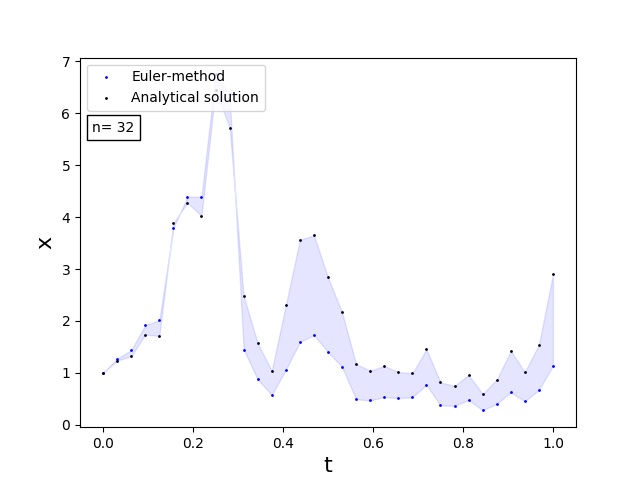
\includegraphics[scale=0.4]{Content/Graphics/SDE_EulerGBM_n_32}
   \end{subfigure}
   \begin{subfigure}{0.49\linewidth} \centering
     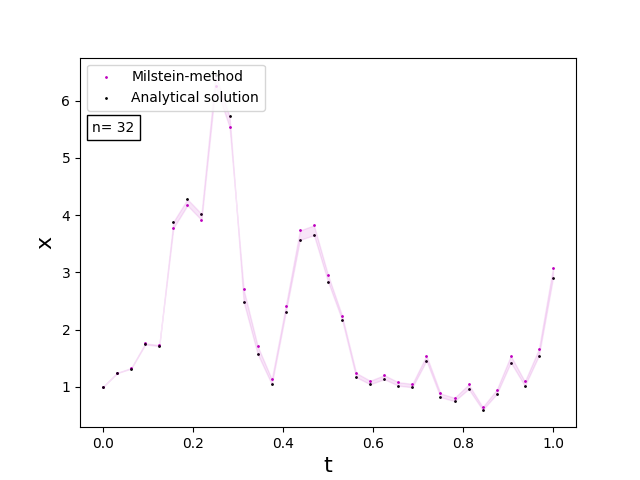
\includegraphics[scale=0.4]{Content/Graphics/SDE_MilsteinGBM_n_32}
   \end{subfigure}
   \begin{subfigure}{0.49\linewidth} \centering
     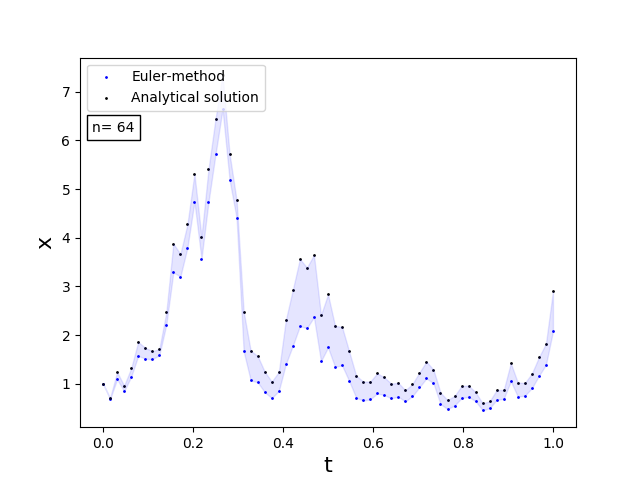
\includegraphics[scale=0.4]{Content/Graphics/SDE_EulerGBM_n_64}
   \end{subfigure}
   \begin{subfigure}{0.49\linewidth} \centering
     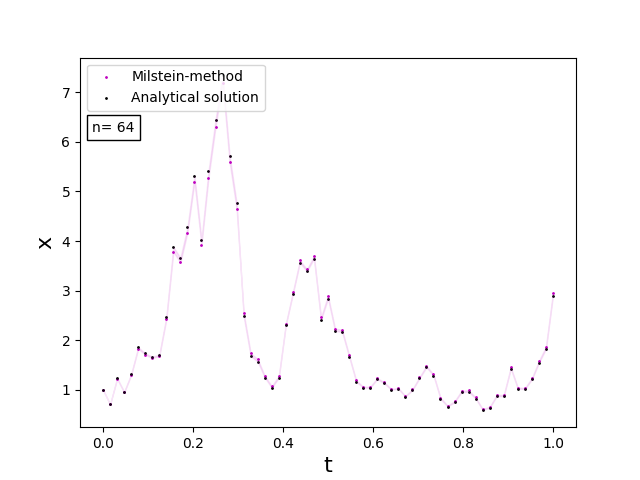
\includegraphics[scale=0.4]{Content/Graphics/SDE_MilsteinGBM_n_64}
   \end{subfigure}
\caption{Approximation (colored dots) of the sample path of the geometric Brownian motion and the true sample path (black dots) for n = 32, 64.}
\end{figure}


We did the same analysis for the Ornstein-Uhlenbeck process. Note that this process has a constant diffusion term (\(b(x)=\sigma\)). Thus the additional term of the Milstein-schem vanishes and the Euler- and the Milstein-scheme give the same results. Indeed the error-bound of the Milstein-scheme also applies to the Euler-Scheme for stochastic differential equations with constant diffusion terms. The Euler-scheme has convergence order 1.0 in this particular case.
In the following figures we can see that both schemes yield the same result:
\vfill
\begin{figure}[!h]
\centering
   \begin{subfigure}{0.49\linewidth} \centering
     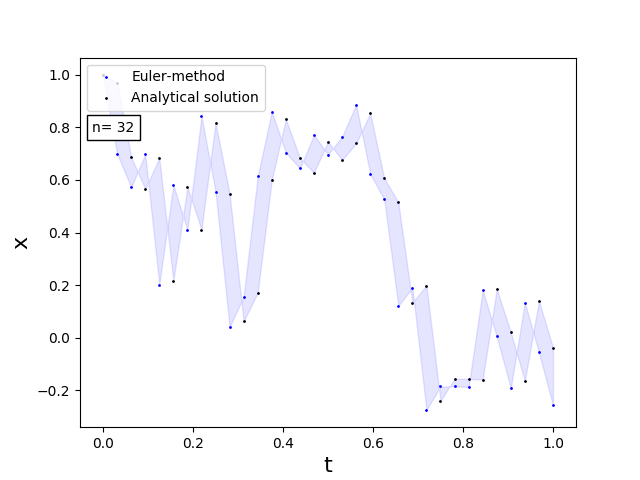
\includegraphics[scale=0.4]{Content/Graphics/SDE_EulerOU_n_32}
   \end{subfigure}
   \begin{subfigure}{0.49\linewidth} \centering
     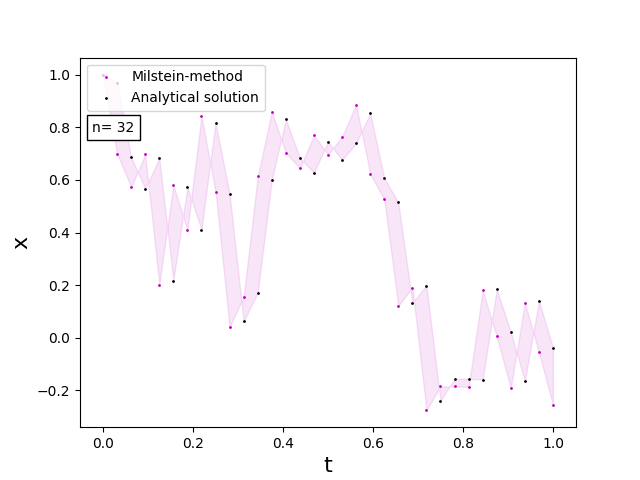
\includegraphics[scale=0.4]{Content/Graphics/SDE_MilsteinOU_n_32}
   \end{subfigure}
   \begin{subfigure}{0.49\linewidth} \centering
     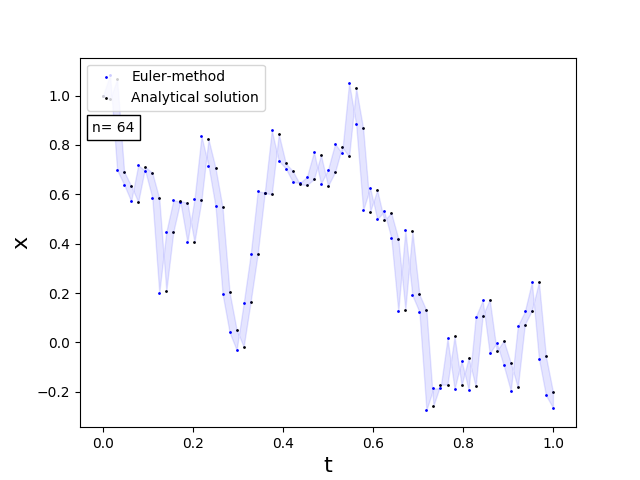
\includegraphics[scale=0.4]{Content/Graphics/SDE_EulerOU_n_64}
   \end{subfigure}
   \begin{subfigure}{0.49\linewidth} \centering
     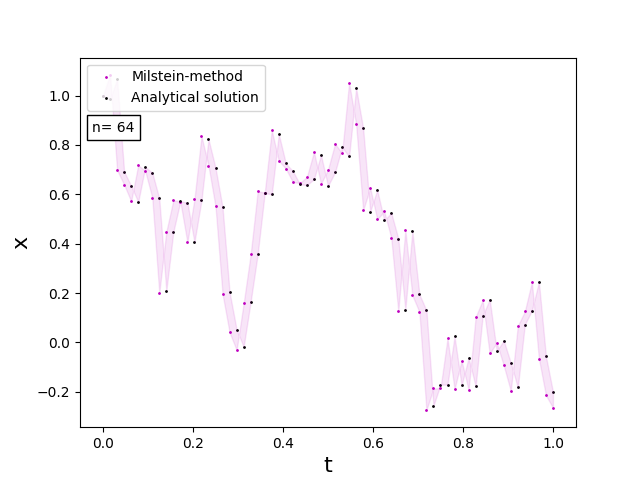
\includegraphics[scale=0.4]{Content/Graphics/SDE_MilsteinOU_n_64}
   \end{subfigure}
\caption{Approximation (colored dots) of the sample path of the Ornstein-Uhlenbeck process and the true sample path (black dots) for n = 32, 64.} 
\end{figure}


The next figures (figure \ref{fig:erroranalysis}) verify that the approximation error \(e_n\) is tending to 0 for increasing step amount n for both, the geometric Brownian motion and the Ornstein-Uhlenbeck process.\\
The approximation errors \(e_n\) have been calculated for \(n = 2^3,\ldots, 2^{10}\). Recall:
\[e_n\coloneqq\mathbb{E}[(X_T - \overline{X}^{n}_{T})^2]^{\frac{1}{2}}.\]

We then took the Monte-Carlo estimates using m = 100'000 simulations for each n. The estimate \(\hat{e}_n\) is defined as follows:
\[\hat{e}_n\coloneqq (\frac{1}{m}\sum_{k=1}^{m}(X_T^k - \overline{X}^{n,k}_{T})^2)^{\frac{1}{2}}\]
for given sample paths \(X_t^1,\ldots, X_t^m\) and the corresponding approximations \(\overline{X}^{n,1}_{t},\ldots,\overline{X}^{n,m}_{t}\).
We did this analysis using the Euler- and the Milstein-scheme and for each step amount n which we set previously.
\begin{figure}[!h]

\centering
   \begin{subfigure}{0.49\linewidth} \centering
     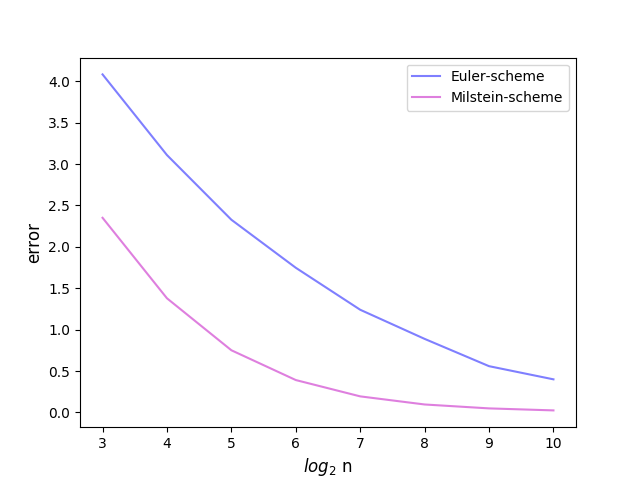
\includegraphics[scale=0.4]{Content/Graphics/ConvergenceEulerMilsteinGBM}
   \end{subfigure}
   \begin{subfigure}{0.49\linewidth} \centering
     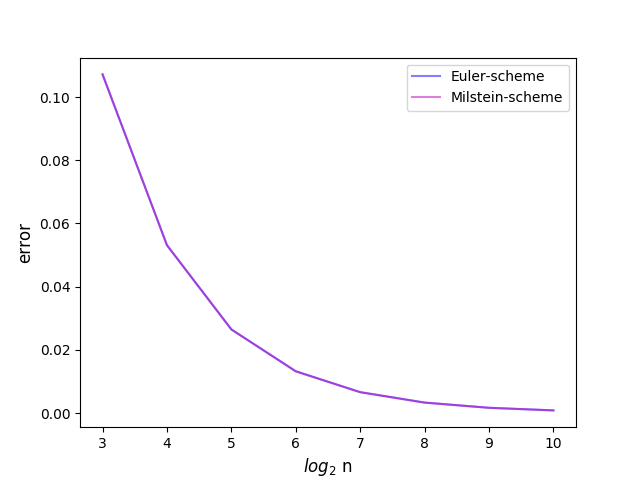
\includegraphics[scale=0.4]{Content/Graphics/ConvergenceEulerMilsteinOU}
   \end{subfigure}
\caption{Monte-Carlo estimates of the approximation error and the step amount n (logarithmized) for the geometric Brownian motion (left) and the Ornstein-Uhlenbeck process (right).} 
\label{fig:erroranalysis}
\end{figure}

The final figures (figure \ref{fig:convergenceanalysis}) show the log-log plot for the estimates of the approximation error and the step amount n. As was discussed in section \ref{erroranalysis} the (absolute value) of the slope of the regression line is an estimate for the convergence order.
The estimated convergence orders for the geometric Brownian motion match the analytical results. (0.5 for the Euler-scheme and 1.0 for the Milstein-Scheme). The same analysis on the Ornstein-Uhlenbeck process yields an order of 1.0 for both schemes.
However this is always the case if the diffusion term of the stochastic differential equation is constant, as we discussed previously. 
Our estimates for the convergence orders are:
\begin{enumerate}[noitemsep,topsep=0mm,labelindent=6mm,leftmargin=*,widest=3.,align=right]
\item Geometric Brownian motion:
\begin{enumerate}[noitemsep,topsep=0mm,labelindent=6mm,leftmargin=*,widest=3.,align=right]
\item Euler: 0.482.
\item Milstein: 0.950. 
\end{enumerate}
\item Ornstein-Uhlenbeck process:
\begin{enumerate}[noitemsep,topsep=0mm,labelindent=6mm,leftmargin=*,widest=3.,align=right]
\item Euler: 1.003.
\item Milstein: 1.003.
\end{enumerate}
\end{enumerate}

\begin{figure}[!h]

\centering
   \begin{subfigure}{0.49\linewidth} \centering
     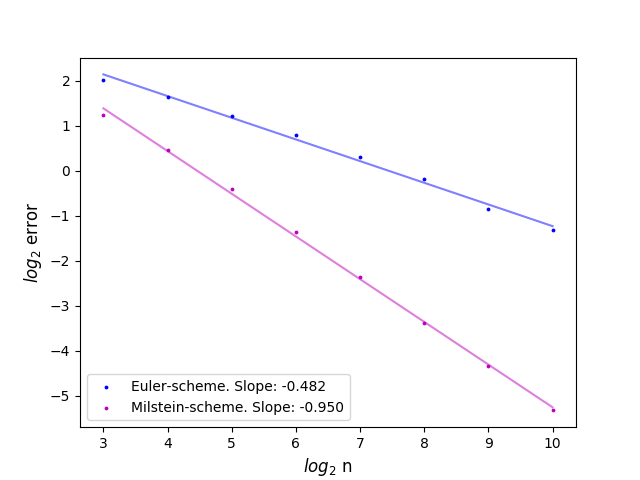
\includegraphics[scale=0.4]{Content/Graphics/Convergence_OrderEulerMilsteinGBM}
   \end{subfigure}
   \begin{subfigure}{0.49\linewidth} \centering
     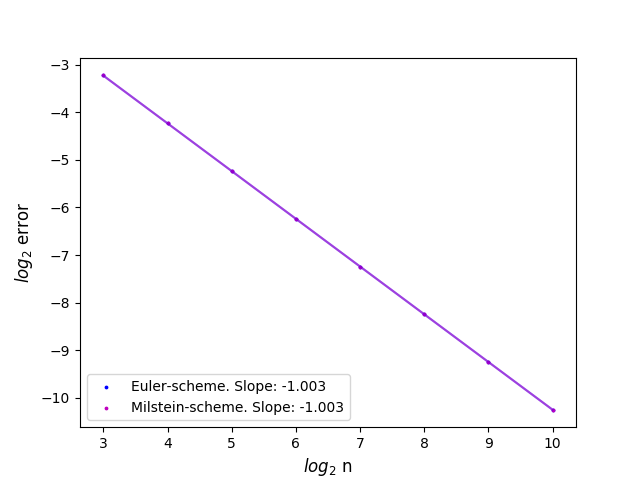
\includegraphics[scale=0.4]{Content/Graphics/Convergence_OrderEulerMilsteinOU}
   \end{subfigure}
\caption{Log-log plot of the approximation error and the step amount n for the geometric Brownian motion (left) and the Ornstein-Uhlenbeck process (right).} 
\label{fig:convergenceanalysis}
\end{figure}
\vfill

\section{Conclusion}

We conclude that even for a low amount of discretization steps n, the Milstein-scheme gives an impressive approximation for the true sample paths. The implementation is not difficult and should always be prefered over the Euler-scheme.
More graphics can be seen in appendix \ref{Graphics}. We also verified the (theoretical) convergence orders numerically.\\

However we remark that the conditions for both schemes (globally Lipschitz) are quite strong and therefore the schemes do not allow for coefficients which do not fulfill these conditions. There are many stochastic differential equations which have non-Lipschitz coefficients. Further research can be done by finding the convergence proofs which works for weaker conditions. Better (in terms of higher convergence order) schemes, if necessary, can be obtained by iteratively applying the It\^o-lemma on the coefficients and by truncating these stochastic Taylor expansions (given that the coefficients are smooth enough). However these higher-order schemes become complex very quickly.\\

One might think that there is also a generalization of the Heun-method for stochastic differential equations, since also the Euler-Maruyama method is a generalization of a well-known method from deterministic analysis. The Heun-method is based on the trapezoid-rule from numerical integration theory. Since we are operating with It\^o stochastic integrals, we cannot apply the trapezoid rule (recall the definition of the It\^o stochastic integral). However there exist implicit schemes and also derivative-free schemes (Runge-Kutta) for stochastic differential equations and we refer to \cite{KloedenPlaten} for their treatment.\\

We end the thesis with the final remark that numerical schemes for stochastic differential equations are obtained in a similair way as their deterministic counterparts. We also used methods which are analogous to the Taylor expansion in order to construct our approximation schemes, by truncating these expansions. However we cannot blindly generalize methods from (deterministic) numerical analysis. We do need to take the stochastic setting into our consideration. In our case, this was the It\^o stochastic calculus.
Therefore it is inevitable to have profound knowledge in stochastic analysis, if one wishes to construct numerical schemes for stochastic differential equations.











